\documentclass[12pt, a4paper]{article}
\usepackage{indentfirst}
\usepackage{graphicx}
\usepackage{url}
\def\UrlBreaks{\do\/\do-}
\usepackage{cite}
\usepackage{float}
\usepackage[font=footnotesize,labelfont=bf]{caption}
\graphicspath{{images/}}
\title{GDPR: Is non-compliance profitable for Meta Platforms, Inc.?}
\author{Stoyan L. Kostadinov}
\date{June 2023}
\begin{document}
\maketitle

\begin{center}
    
\includegraphics[width=0.3\textwidth]{fontys-logo}
\end{center}

\begin{abstract}
    This paper investigates the financial implications of General Data
    Protection Regulation (GDPR) fines on \textit{Meta Platforms, Inc.}
    (formerly \textit{Facebook, Inc.}). By examining net income, revenue, stock
    price, volume of shares traded, and average revenue per person, the study
    assesses the relationship between GDPR penalties and Meta's financial
    performance. The findings suggest that GDPR fines did not have any impact,
    with investor confidence remaining stable, revenue unaffected, and net
    income declining in line with other tech companies. However, a slight
    decline in average revenue per person in Europe compared to the US is
    observed. Further research is needed to explore legal expenses, reputation,
    and user perception related to GDPR non-compliance.
\end{abstract}

\subsection*{Keywords}

GDPR, Facebook, Meta, profit, non-compliance, privacy, financial impact

\section*{Introduction}

In the recent years, the increasing usage of the Internet has lead to a rapid
expansion of data collection and processing\cite{khan2014big}. As concerns
regarding data privacy and protection grew, the European Union (EU) implemented
the General Data Protection Regulation (GDPR) in May
2018\cite{greengard2018weighing, historyGdpr}.

GDPR aimed to safeguard the privacy rights of individuals within the EU by
regulating the collection, storage, and transfer of personal
data\cite{historyGdpr}. Notably, data should be collected for specified,
explicit and legitimate purposes\cite{europeanParliamentGdprArticle5} and data
can be transferred outside the EU if general data processing principles are in
place \cite{europeanParliamentGdprArticle44}. Compliance with GDPR has become a
critical issue for big-tech companies, which often handle massive amounts of
user data.

One of those companies is \textit{Meta Platforms, Inc.} (formerly
\textit{Facebook, Inc.}), which has been fined numerous times for GDPR
violations\cite{mrevzar2023analysis}. This has raised questions about the impact
of GDPR on \textit{Meta's} performance.

The goal of this paper is to investigate the financial impact of GDPR
non-compliance on \textit{Meta Platforms, Inc.} and to determine whether it is
profitable for the company to continue violating the regulations.

\section*{Method}

All numerical data about \textit{Meta Platforms, Inc.} has been gathered from
the official \textit{Meta Investor Relations} website\cite{fbMetaFinancials} -
\textbf{Balance Sheets}, \textbf{Income Statements} and \textbf{Form 10-Q}.
Stock performance data has been gathered from the official \textit{Yahoo!
Finance} website\cite{stockPrice}.

GDPR fines imposed on \textit{Meta Platforms, Inc.} have been gathered from the
\textit{GDPR Enforcement Tracker}
website\cite{enforcementtrackerGDPREnforcement} and filtered to include fines
imposed on their family of applications (\textbf{\textit{Facebook}},
\textbf{\textit{WhatsApp}}, \textbf{\textit{Instagram}}) and
\textbf{\textit{Meta Platforms, Inc.}} itself.

\subsection*{Inclusion criteria}

\begin{itemize}
    \item Articles published in English
    \item Articles published after 2010
    \item Data about GDPR fines above 1 million EUR
    \item Data about \textit{Meta Platforms, Inc.} financials
    \item Data between 2018 and 2023
\end{itemize}

\subsection*{Exclusion criteria}

\begin{itemize}
    \item Articles published in languages other than English
    \item Articles published before 2010
    \item Data that is about GDPR fines below 1 million EUR
    \item Data that is not about \textit{Meta Platforms, Inc.} financials
    \item Data before 2018
\end{itemize}

\subsection*{Ethical considerations}

This study is approved by \textit{Fontys University of Applied Sciences,
Eindhoven, The Netherlands}. All data is collected from publicly available
sources and no personal data is collected. The author is not affiliated with
\textit{Meta Platforms, Inc.} or any other company mentioned in this study.

\section*{Results}

\subsection*{GDPR Fines}

\begin{figure}[H]
    \centering
    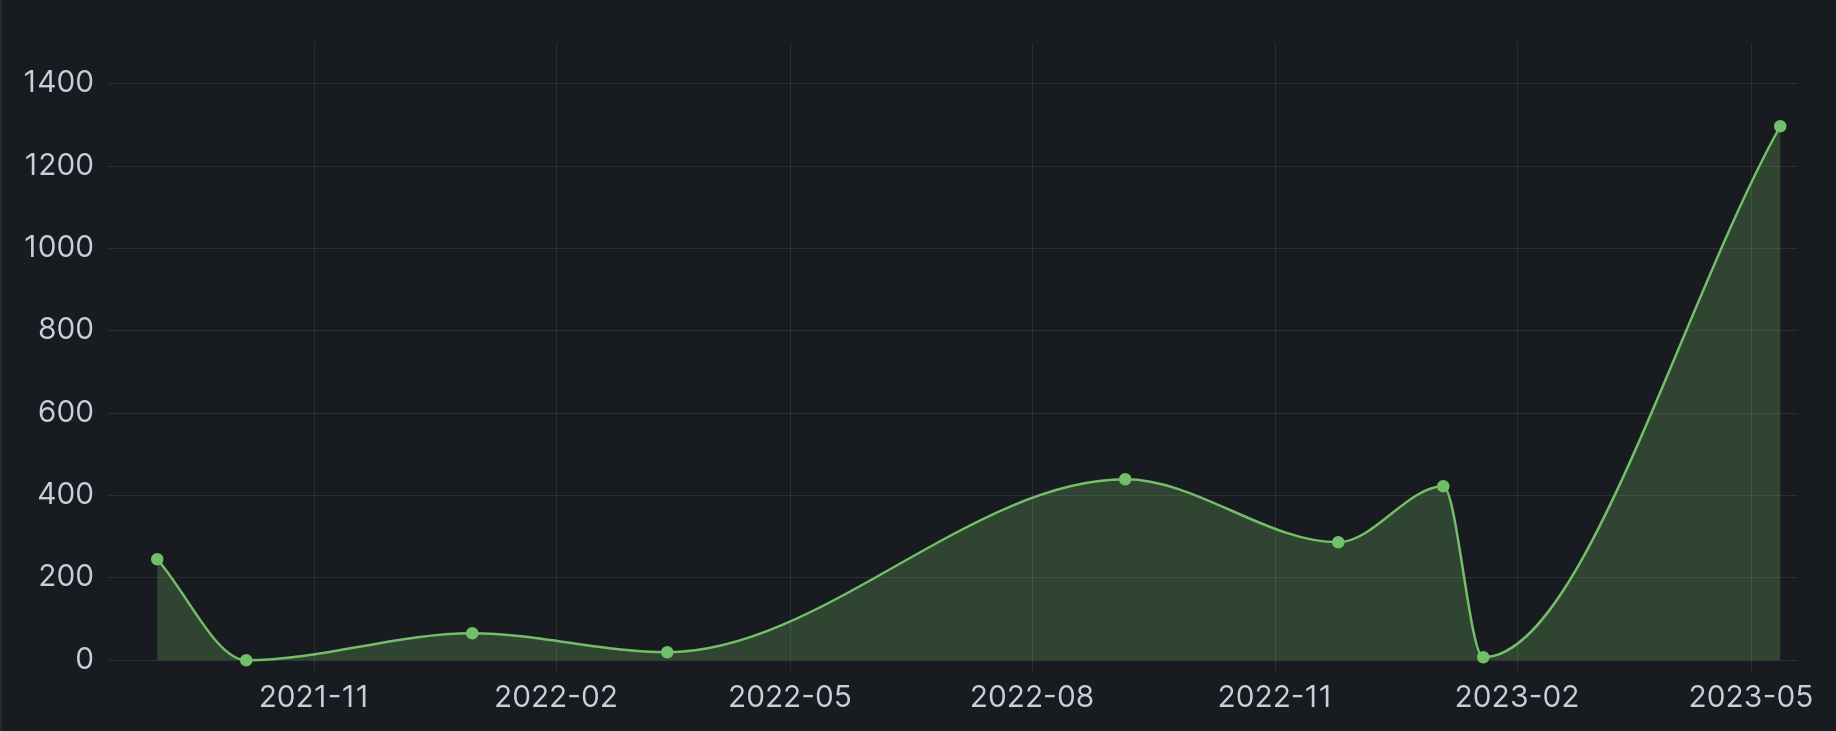
\includegraphics[width=1.00\textwidth]{monetarial-amount-of-gdpr-fines}
    \caption{Monetarial amount of fines issued to Meta Platforms, Inc.(in
    millions of
    \$)\cite{gdprFine1,gdprFine2,gdprFine3,gdprFine4,gdprFine5,gdprFine6,gdprFine7,gdprFine8,gdprFine9}}
    \label{fig:amount-of-gdpr-fines}
\end{figure}

% \begin{figure}[H] \centering
%     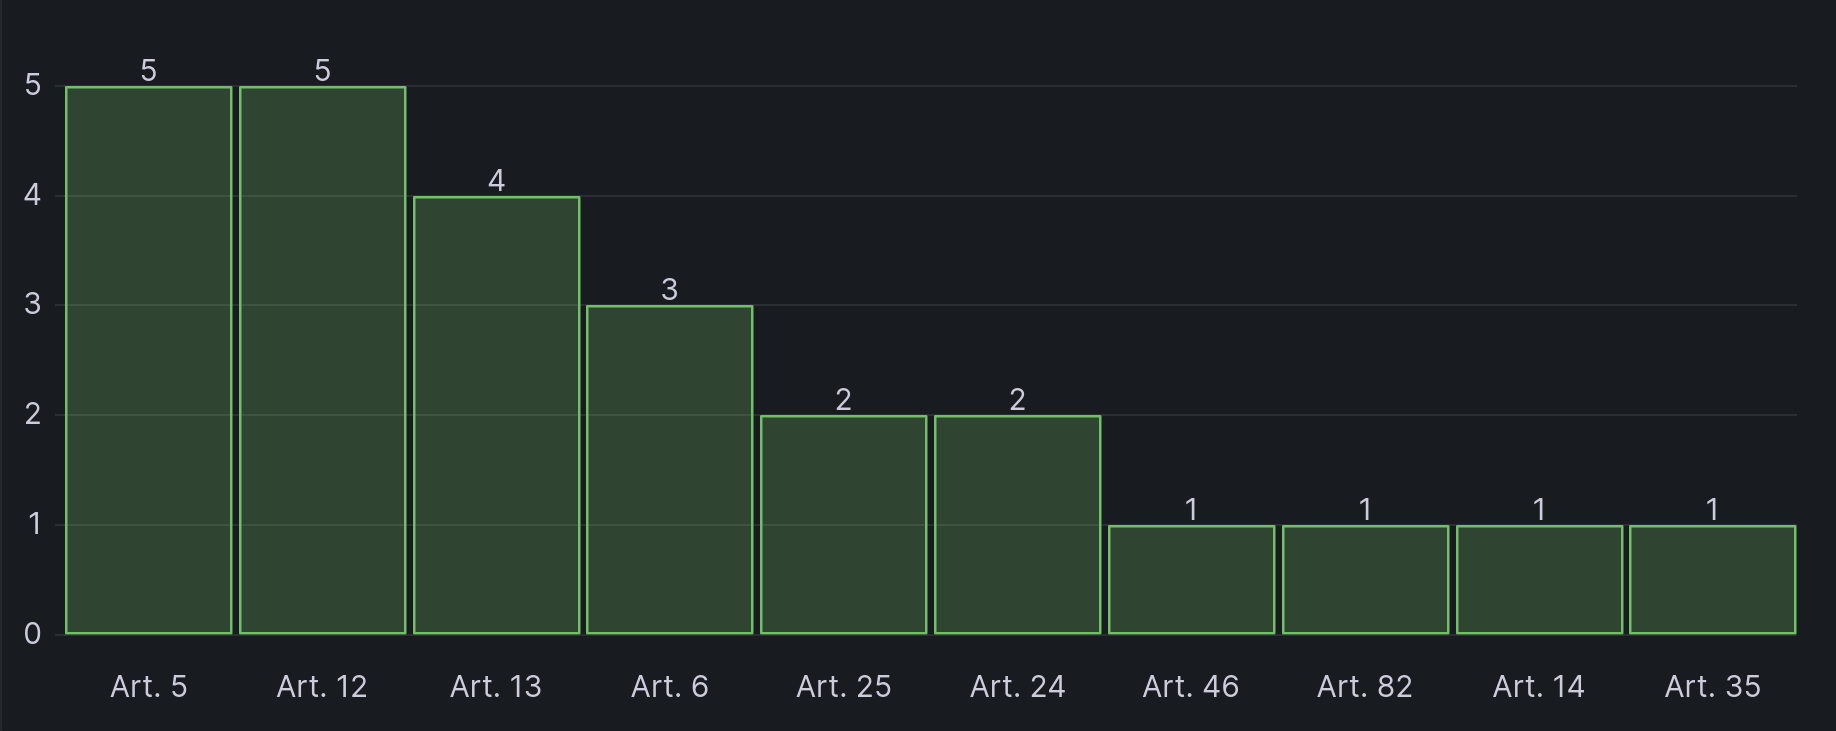
\includegraphics[width=1.00\textwidth]{violations-by-article}
%     \caption{Number of violations by GDPR
%     article\cite{gdprFine1,gdprFine2,gdprFine3,gdprFine4,gdprFine5,gdprFine6,gdprFine7,gdprFine8,gdprFine9}}
%     \label{fig:violations-by-article} \end{figure}

\subsection*{Financials}

\begin{figure}[H]
    \centering
    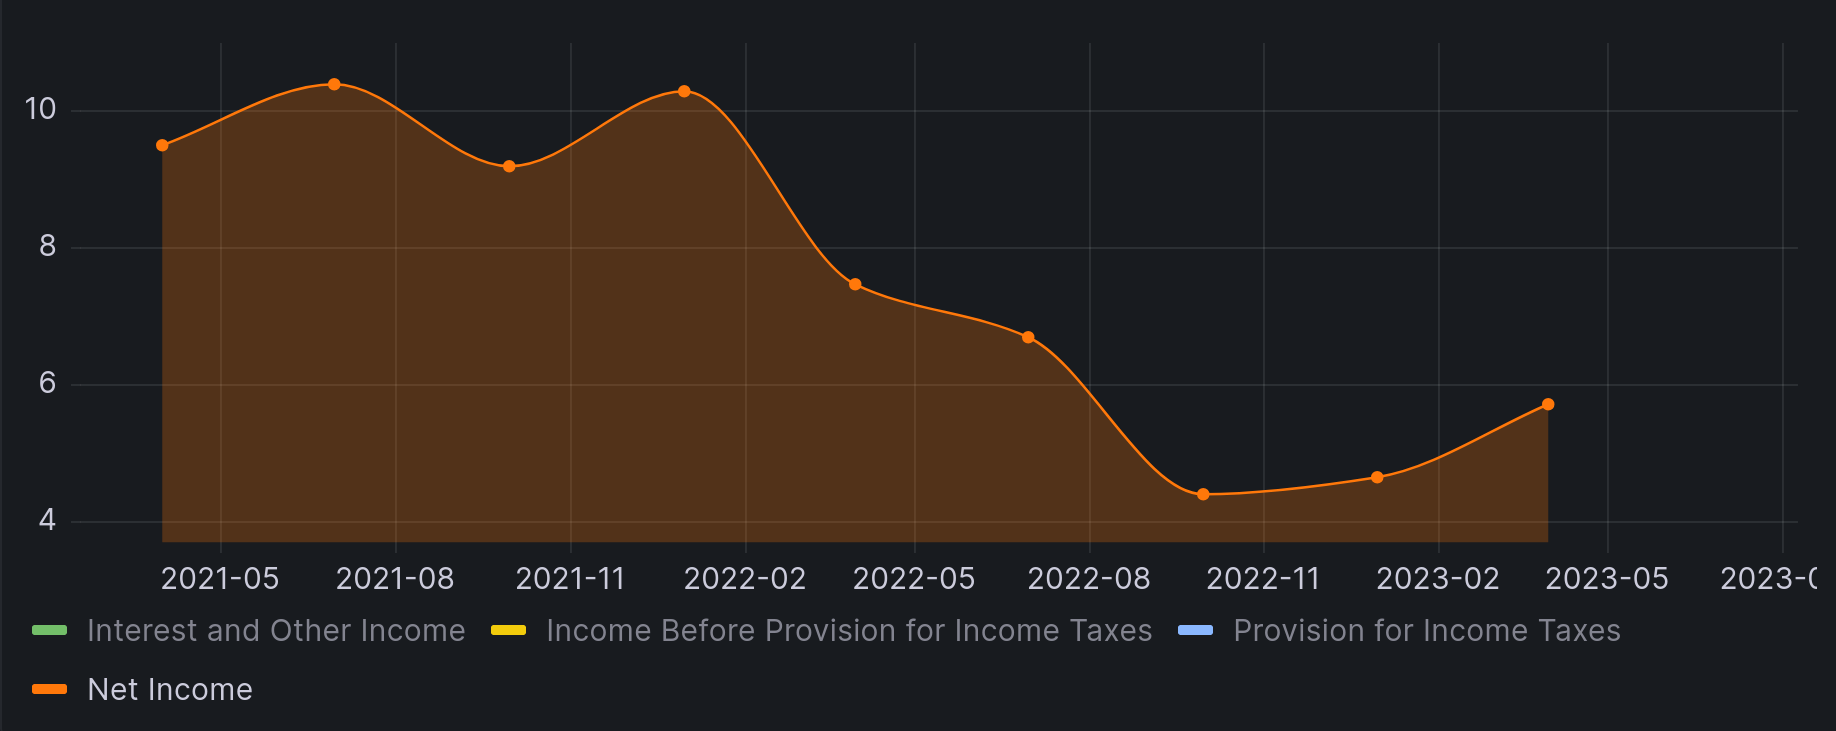
\includegraphics[width=1.00\textwidth]{net-income}
    \caption{Net Income of Meta Platforms, Inc.(in billions of
    \$)\cite{2023q1,2020q4,2020q3,2020q2,2020q1,2019q4,2019q3,2019q2,2019q1,2018q4,2018q3,2018q2}}
    \label{fig:net-income}
\end{figure}

\begin{figure}[H]
    \centering
    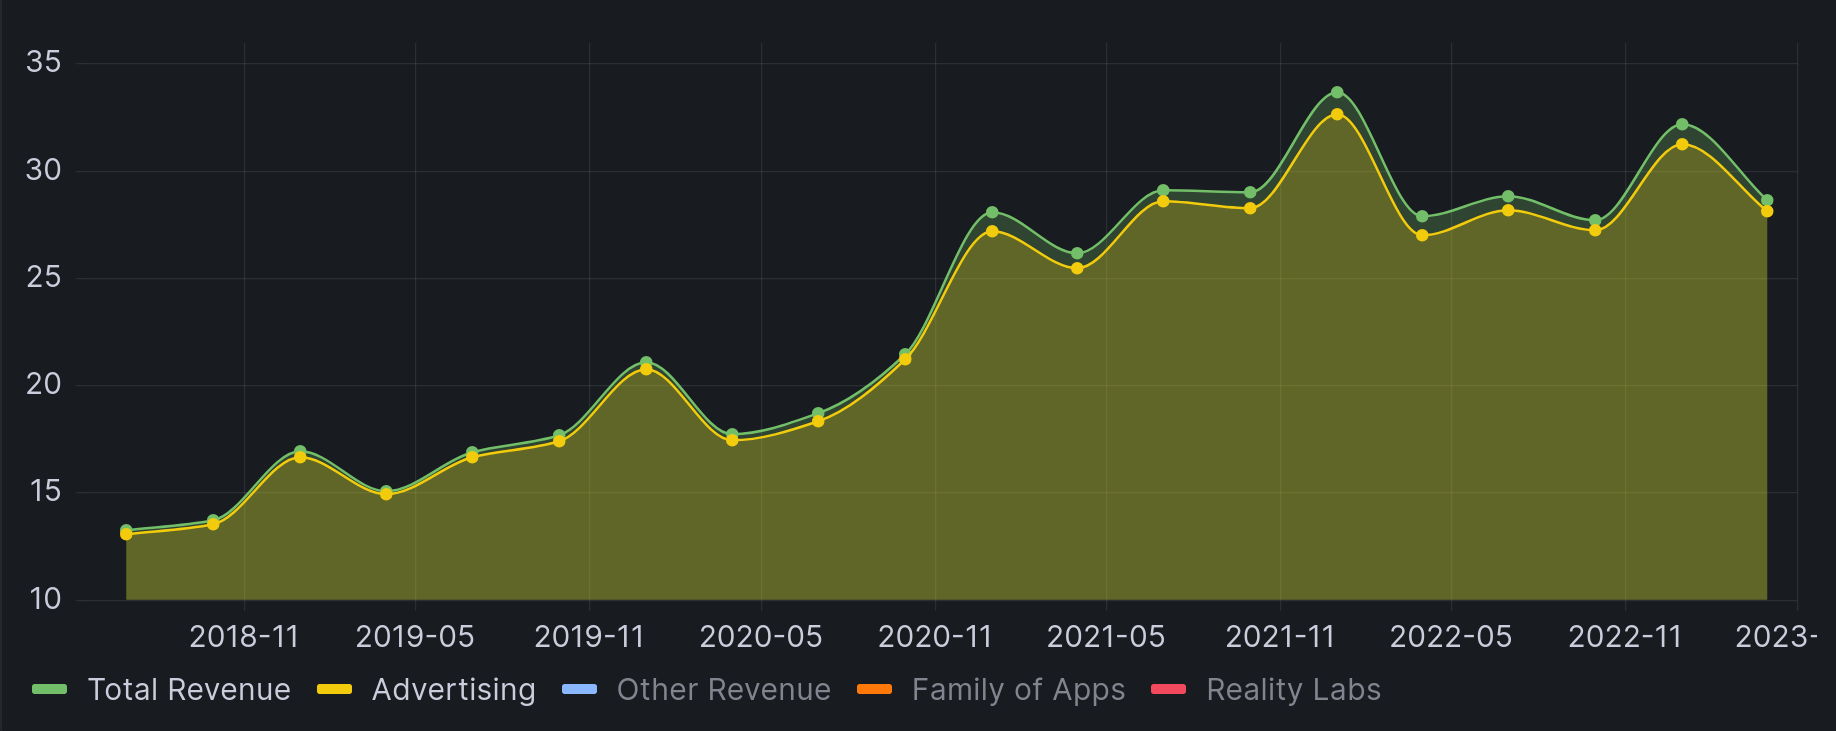
\includegraphics[width=1.00\textwidth]{revenue}
    \caption{Revenue of Meta Platforms, Inc.(in billions of
    \$)\cite{2023q1,2020q4,2020q3,2020q2,2020q1,2019q4,2019q3,2019q2,2019q1,2018q4,2018q3,2018q2}}
    \label{fig:revenue}
\end{figure}

\subsection*{Investor Confidence and Stock Performance}

\begin{figure}[H]
    \centering
    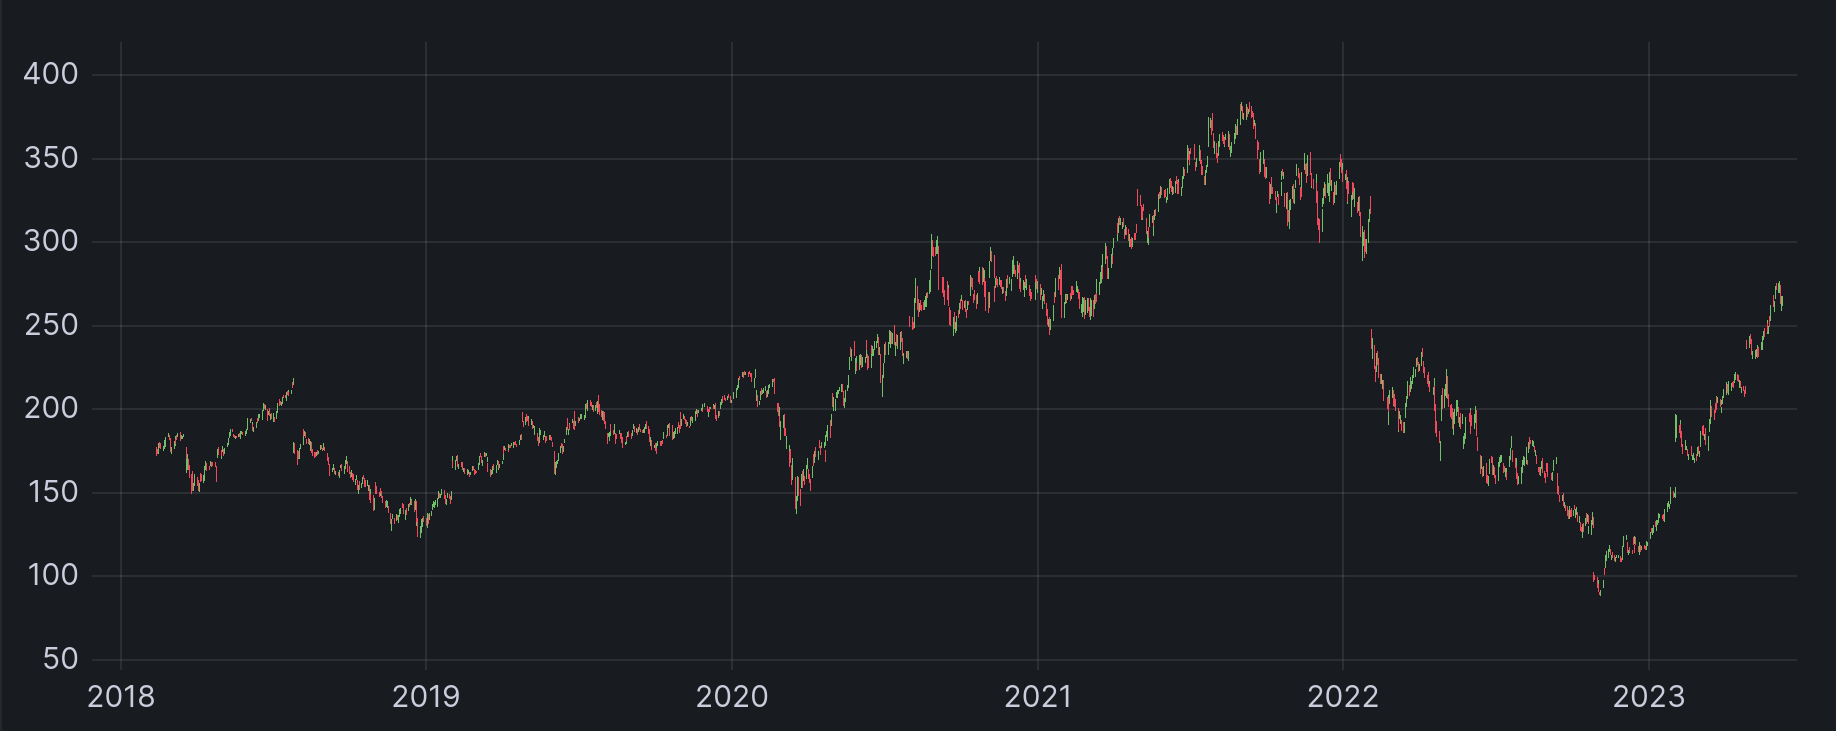
\includegraphics[width=1.00\textwidth]{stock-price}
    \caption{Stock Price Performance of Meta Platforms, Inc. (META) (in
    \$)\cite{stockPrice}}
    \label{fig:stock-price}
\end{figure}

\begin{figure}[H]
    \centering
    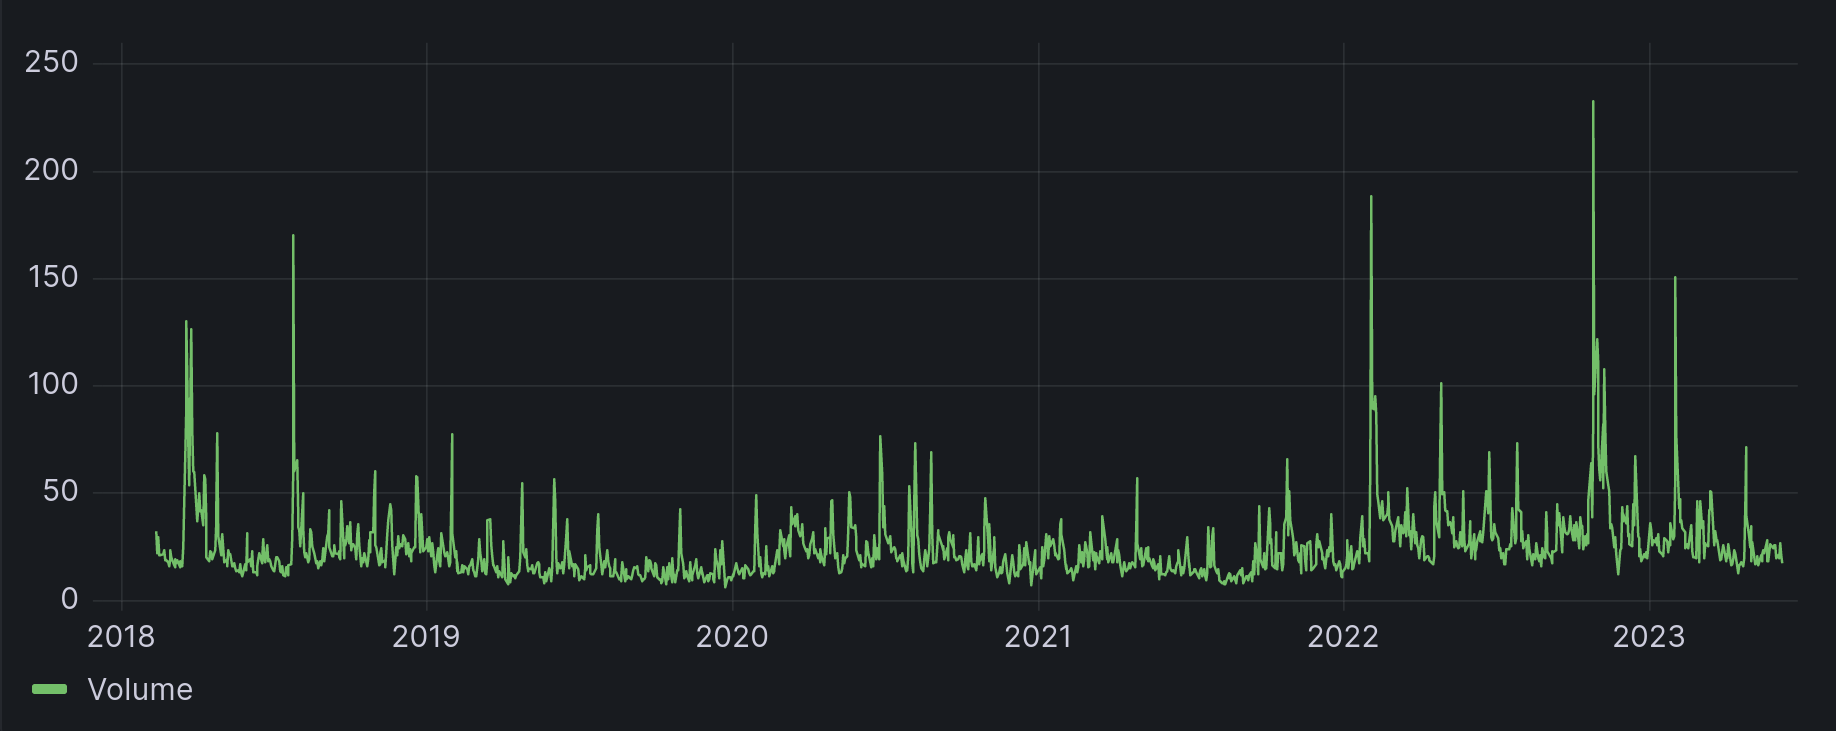
\includegraphics[width=1.00\textwidth]{volume}
    \caption{Volume of Meta Platforms, Inc. (META) (in millions of
    shares)\cite{stockPrice}}
    \label{fig:volume}
\end{figure}

\subsection*{Advertising}

\begin{figure}[H]
    \centering
    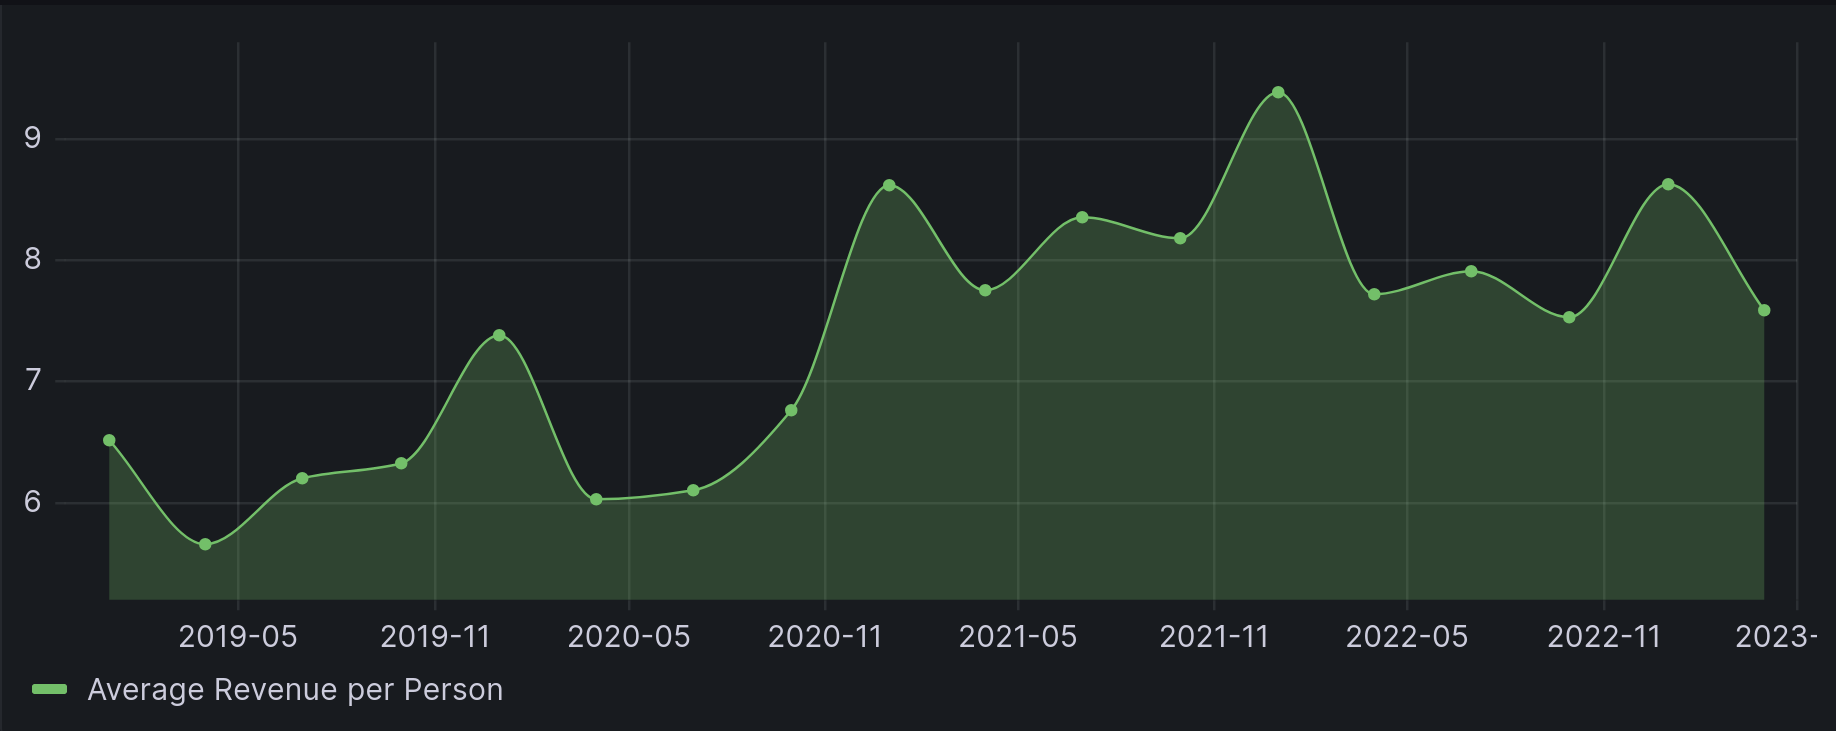
\includegraphics[width=1.00\textwidth]{family-revenue-per-person}
    \caption{Family Revenue per Person (FRP) of Meta Platforms,
    Inc.\cite{2023q1,2021q2Slides,2019q4Slides}}
    \label{fig:family-revenue-per-person}
\end{figure}

\begin{figure}[H]
    \centering
    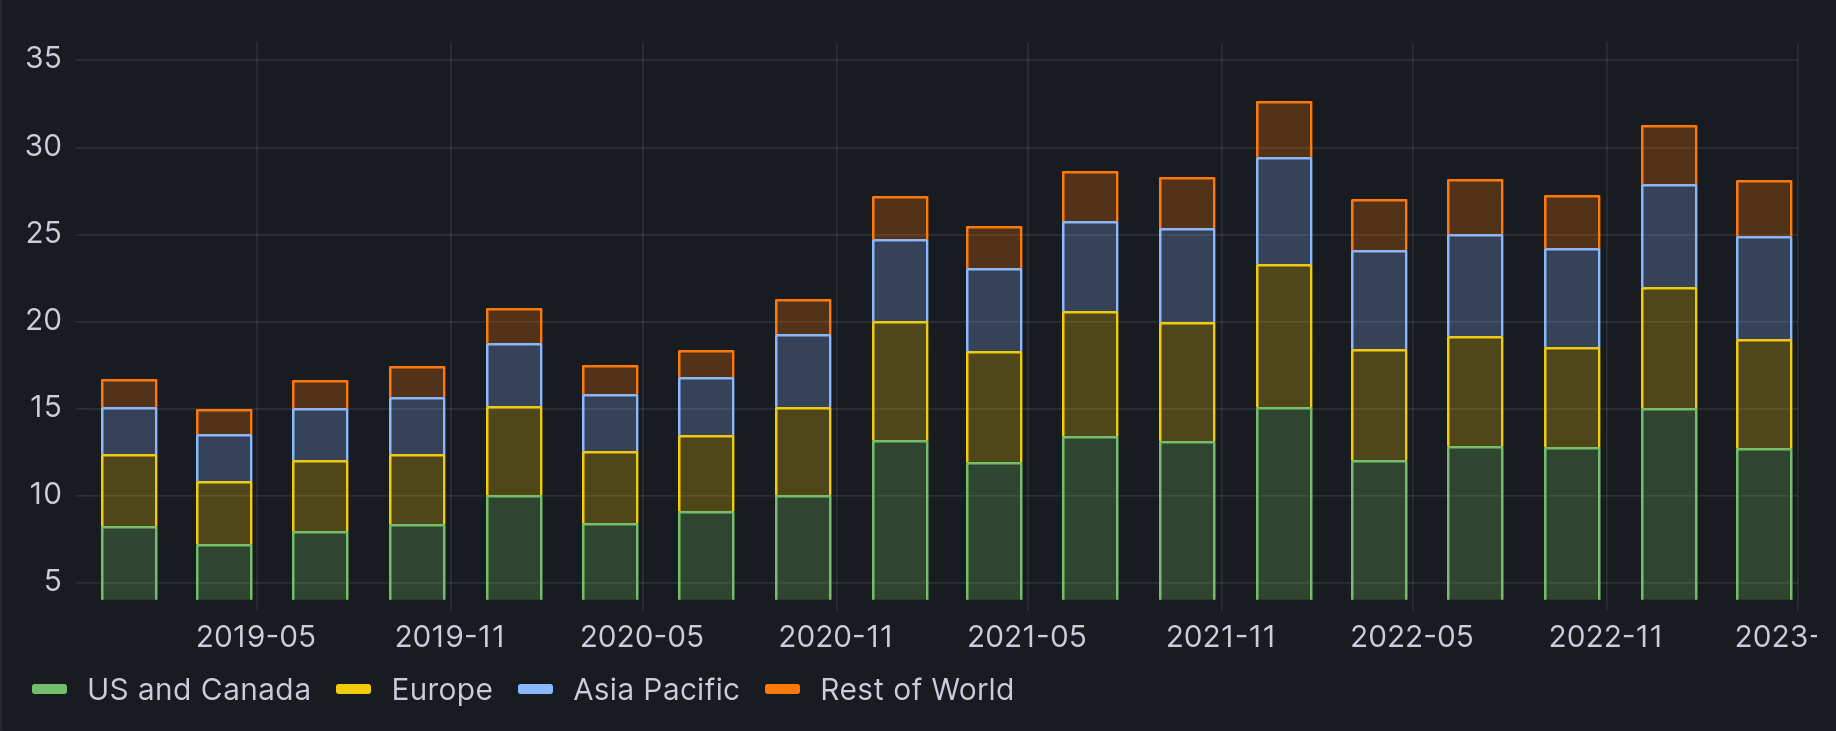
\includegraphics[width=1.00\textwidth]{advertising-revenue-by-user-geography}
    \caption{Advertising Revenue by User Geography of Meta Platforms, Inc.(in
    billions of \$)\cite{2023q1,2021q2Slides,2019q4Slides}}
    \label{fig:advertising-revenue-by-user-geography}
\end{figure}

\subsection*{User Base and User Engagement}

\begin{figure}[H]
    \centering
    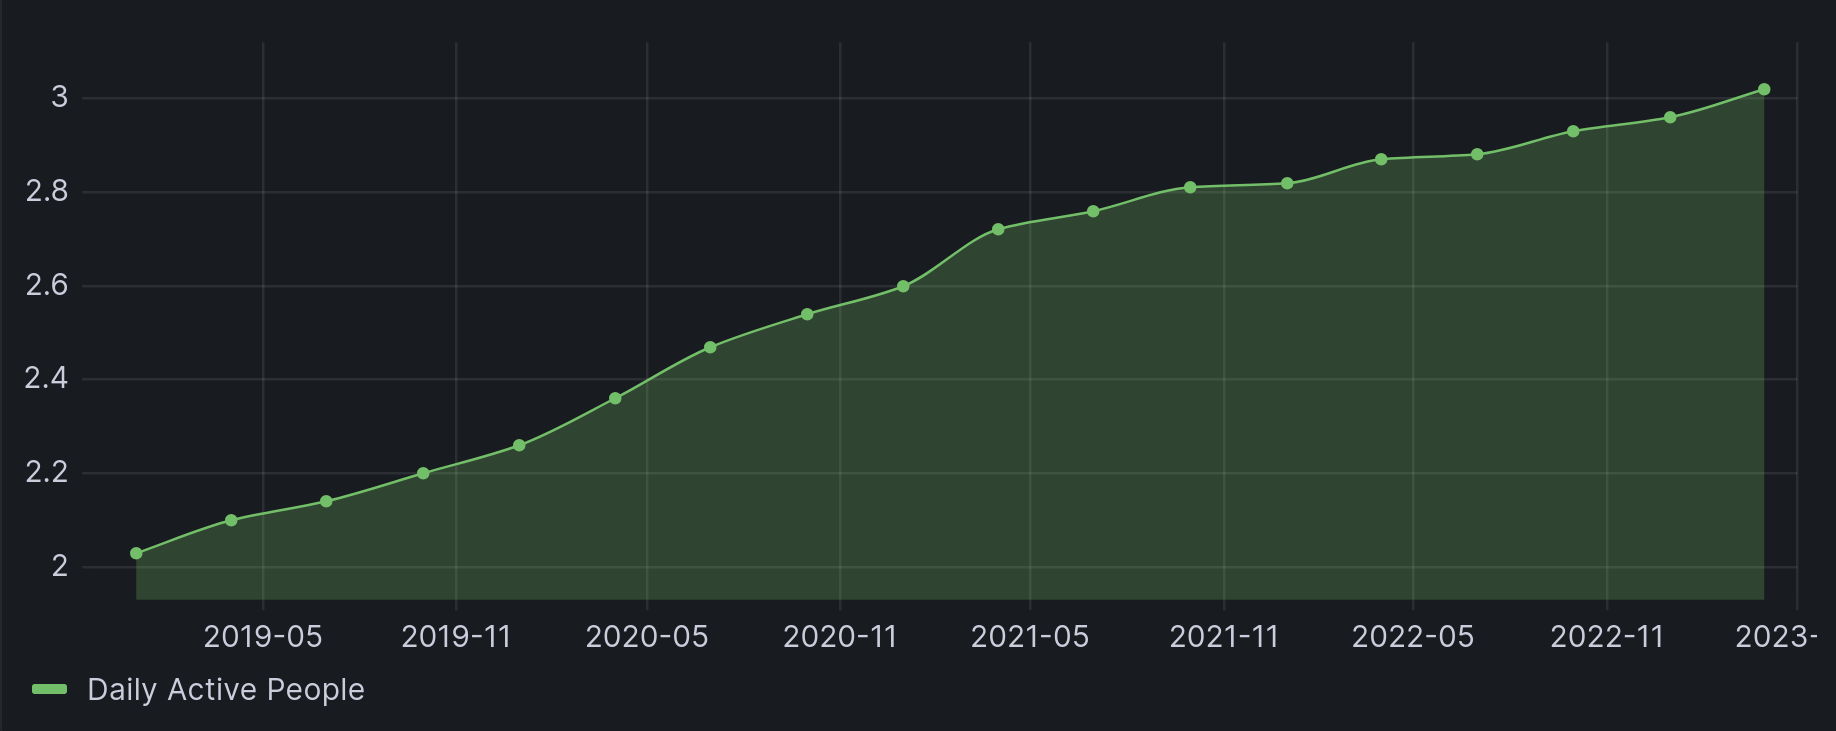
\includegraphics[width=1.00\textwidth]{family-dap}
    \caption{Family Daily Active People (FDAP) of Meta Platforms, Inc.(in
    billions)\cite{2023q1,2021q2Slides,2019q4Slides}}
    \label{fig:family-dap}
\end{figure}

\begin{figure}[H]
    \centering
    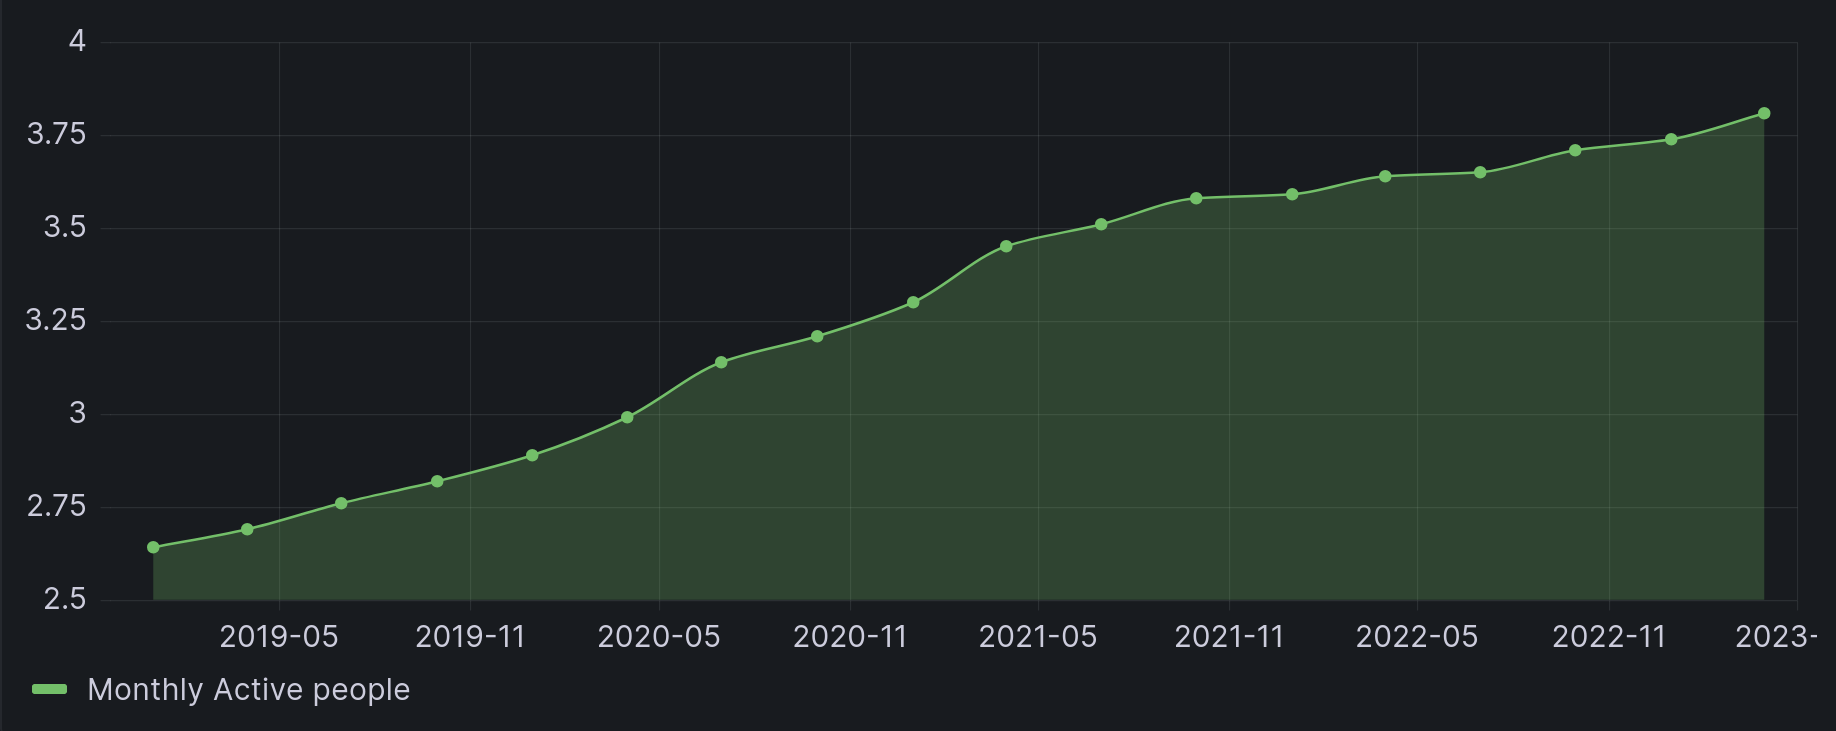
\includegraphics[width=1.00\textwidth]{family-map}
    \caption{Family Monthly Active People (FMAP) of Meta Platforms, Inc.(in
    billions)\cite{2023q1,2021q2Slides,2019q4Slides}}
    \label{fig:family-map}
\end{figure}

\begin{figure}[H]
    \centering
    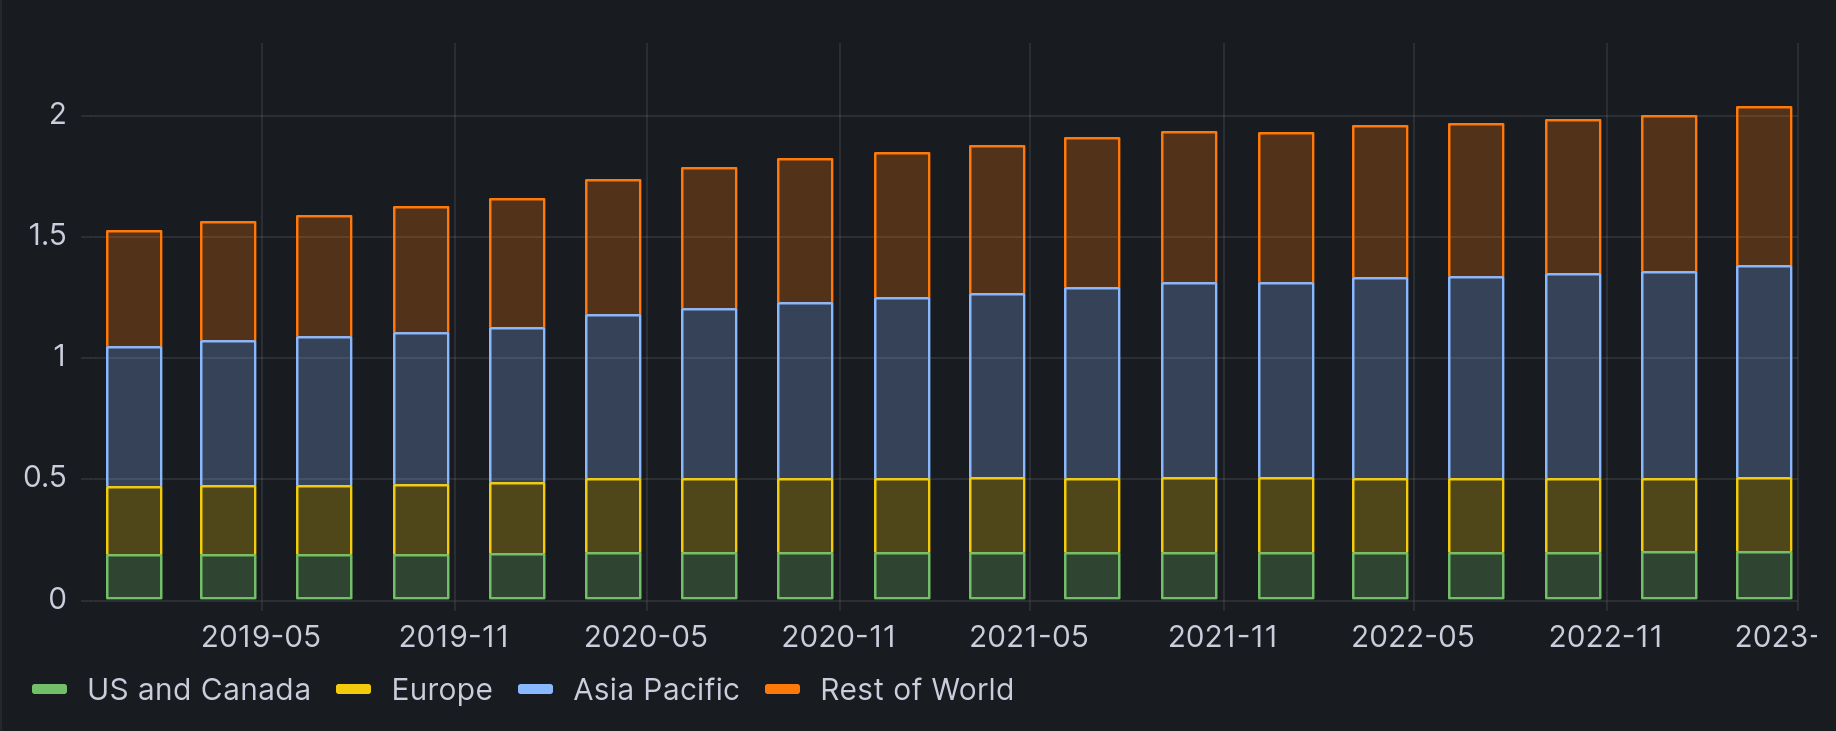
\includegraphics[width=1.00\textwidth]{facebook-dau}
    \caption{Facebook Daily Active Users (FDAU) by Geographical Location of Meta
    Platforms, Inc.(in billions)\cite{2023q1,2021q2Slides,2019q4Slides}}
    \label{fig:facebook-dau}
\end{figure}

\begin{figure}[H]
    \centering
    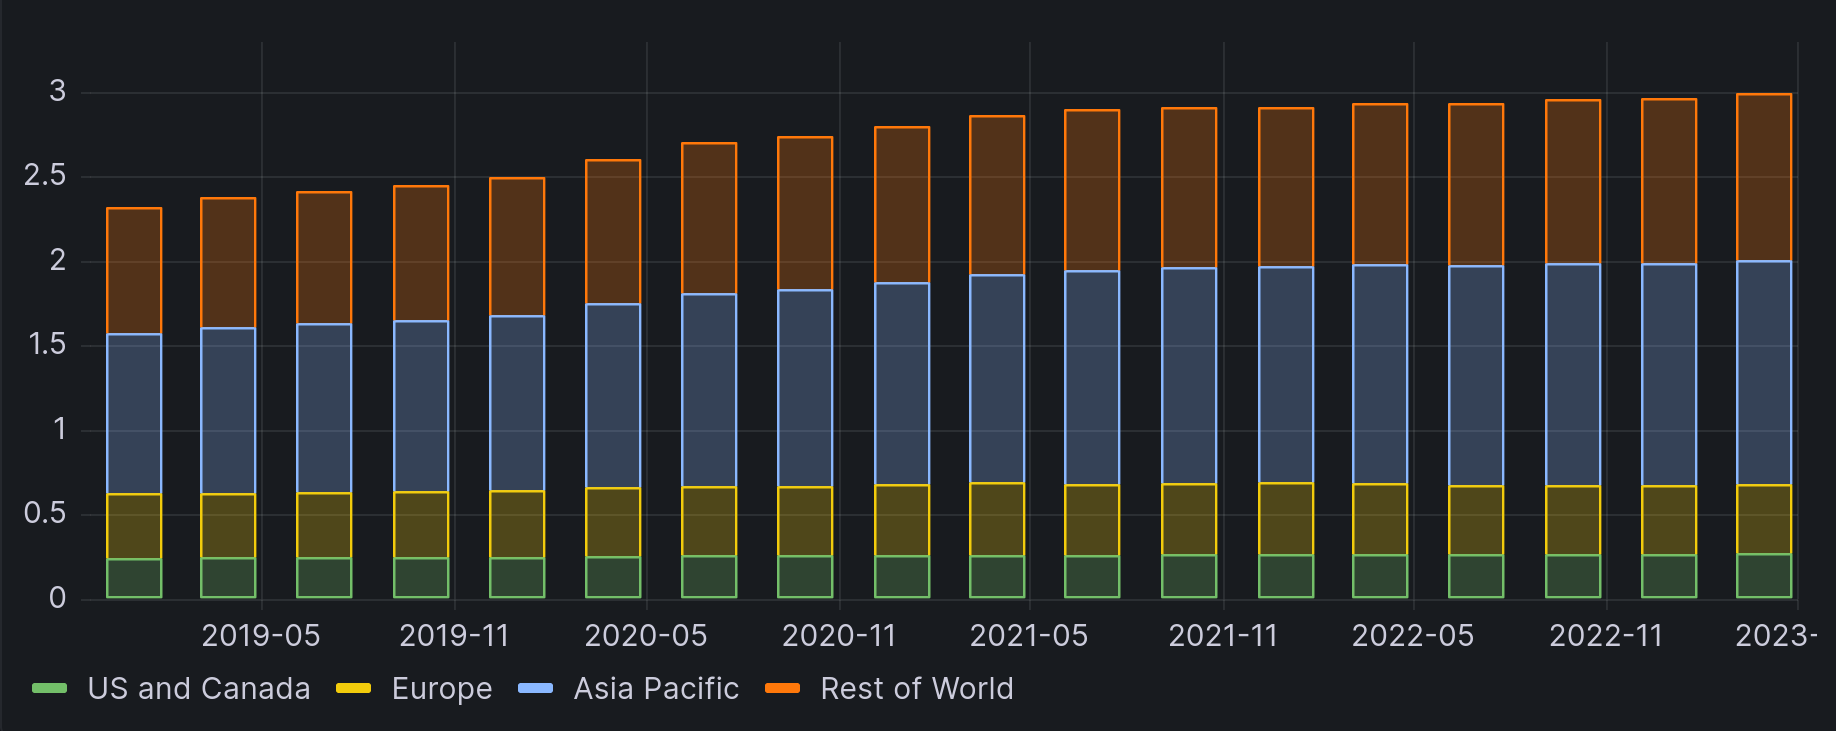
\includegraphics[width=1.00\textwidth]{facebook-mau}
    \caption{Facebook Monthly Active Users (FMAU) by Geographical Location of
    Meta Platforms, Inc.(in billions)\cite{2023q1,2021q2Slides,2019q4Slides}}
    \label{fig:facebook-mau}
\end{figure}

\section*{Discussion}
% Geography page 46 - advertising !!!


% state the results of each graph state what I want the readers to see from each
% graph

% connections

Comparing net income and monetarial amount of GDPR fines shows little to no
signs of correlation. Since the first GDPR fine was issued in 2021 as displayed
in Figure \ref{fig:amount-of-gdpr-fines}, the net income has decreased by 46.7\%
as displayed in Figure \ref{fig:net-income}. However, this can be attributed to
other macroeconomic factors because the net income of other large technology
companies such as \textit{Amazon.com, Inc.} and \textit{Alphabet, Inc.}, has
also decreased in a similar fashion\cite{amznNetIncome,googleNetIncome}. Figure
\ref{fig:rel-fines-net-income} below shows a comparison between both figures.

\begin{figure}[H]
    \centering
    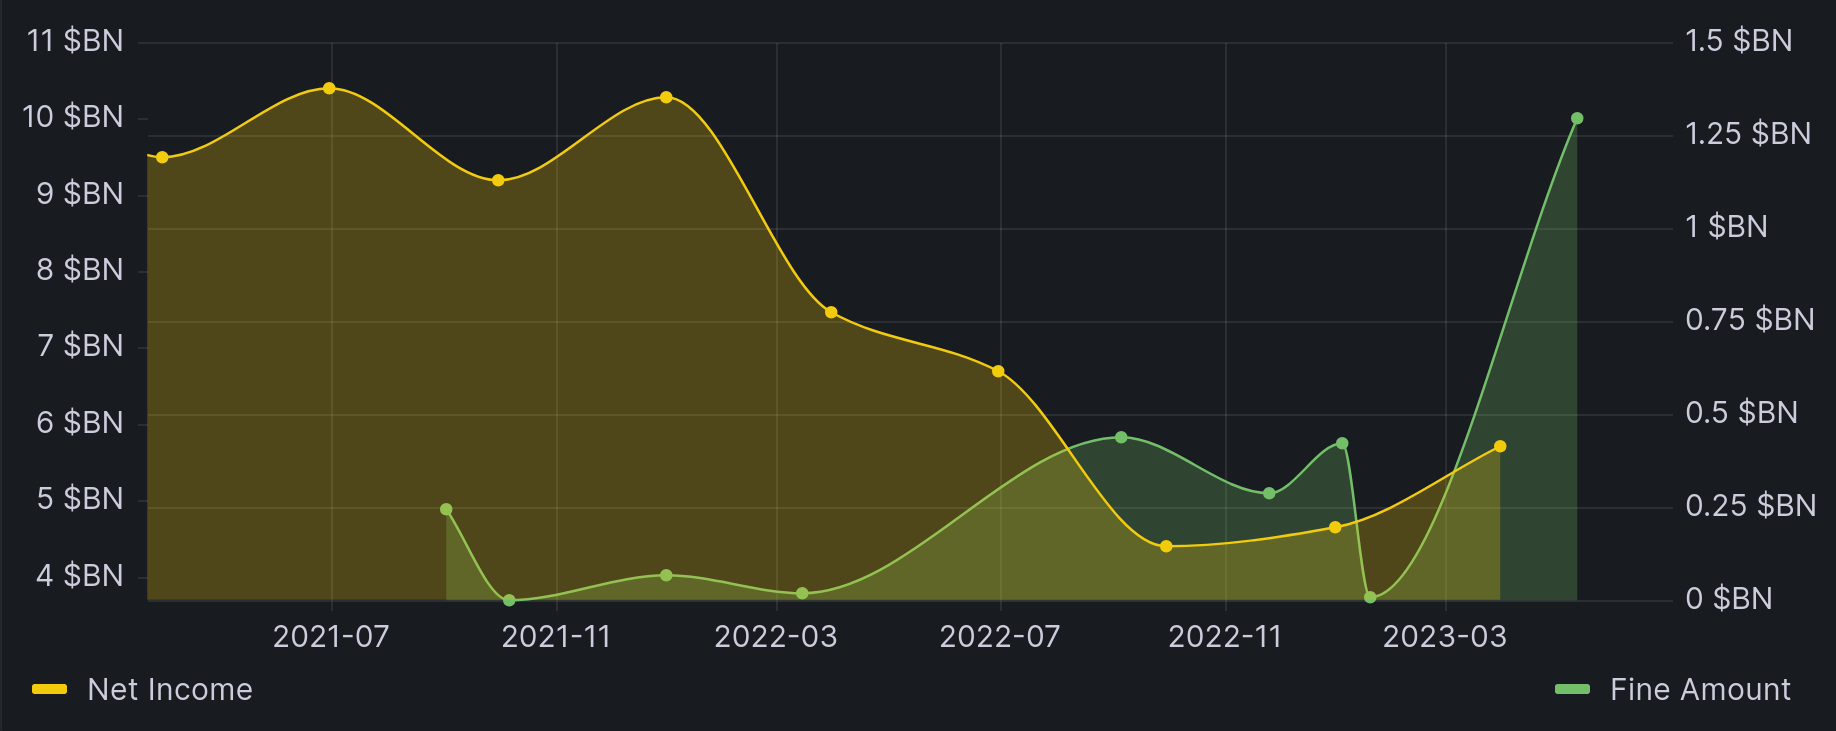
\includegraphics[width=1.00\textwidth]{rel-fines-net-income}
    \caption{Comparison between Net Income and Monetarial Amount of GDPR Fines}
    \label{fig:rel-fines-net-income}
\end{figure}

Similarly, the revenue is not affected as well. Figure
\ref{fig:rel-fines-revenue} below shows a comparison between revenue and the
monetarial amount of GDPR fines.

\begin{figure}[H]
    \centering
    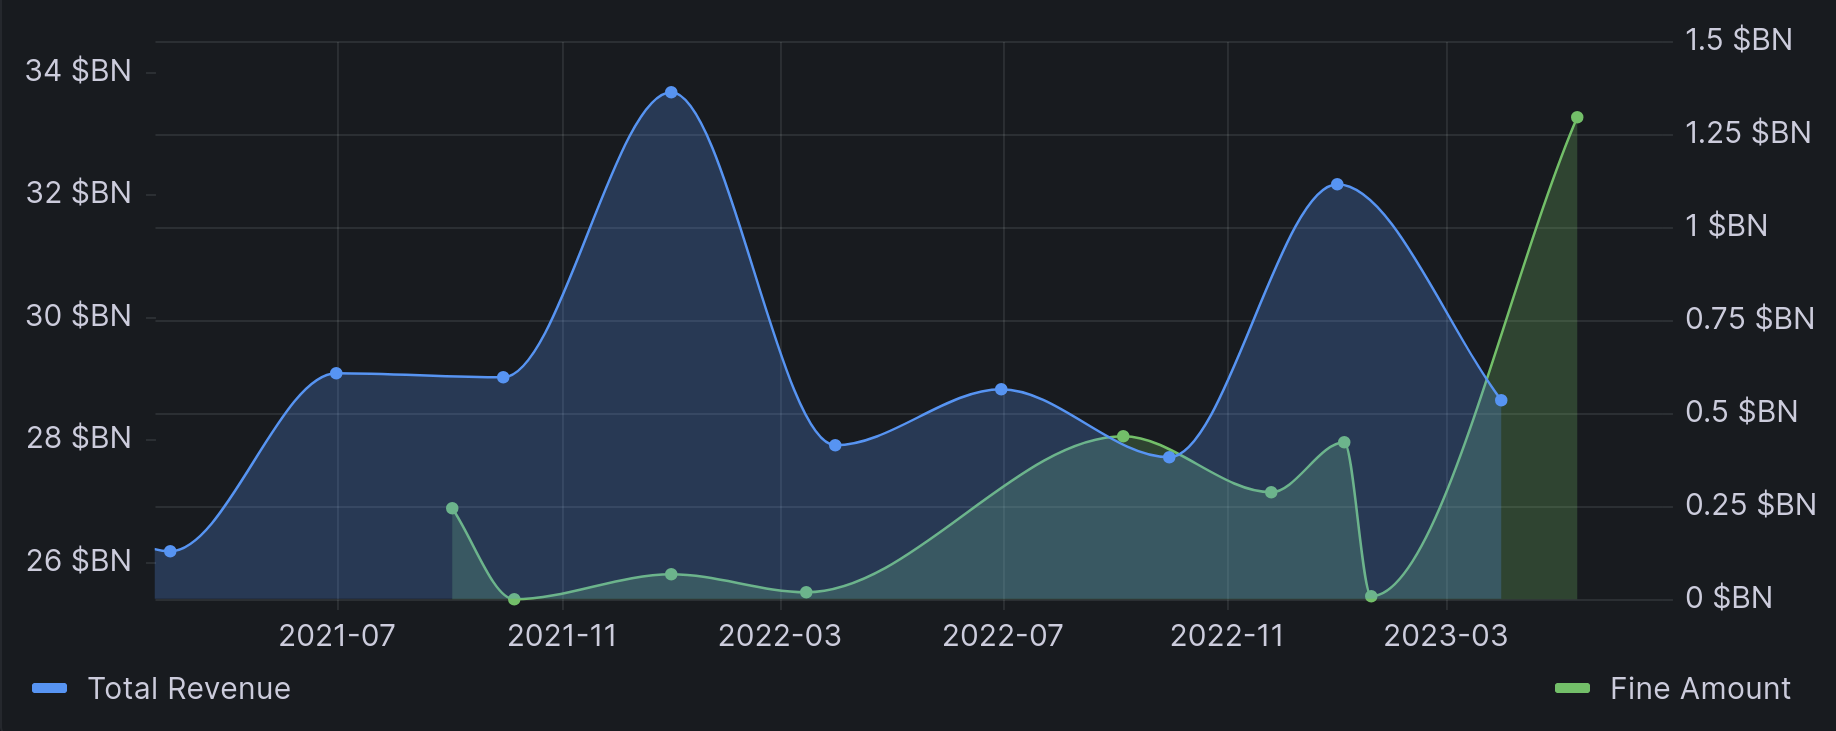
\includegraphics[width=1.00\textwidth]{rel-fines-revenue}
    \caption{Comparison between Revenue and Monetarial Amount of GDPR Fines}
    \label{fig:rel-fines-revenue}
\end{figure}

Figure \ref{fig:stock-price} shows that the first GDPR fine might have had a
negative impact on the stock price, but subsequent more severe fines did not. In
fact, the latest record-breaking fine of \$1.2 billion shows an opposite trend
where the stock price continues to increase from \$234 to \$265 by the time this
report was written. It is worth noting that the stock price reaction might
experience a delay based on whether the fine will be imposed or not as
\textit{Meta} is arguing against the fine \cite{metaArgueFine}.

\begin{figure}[H]
    \centering
    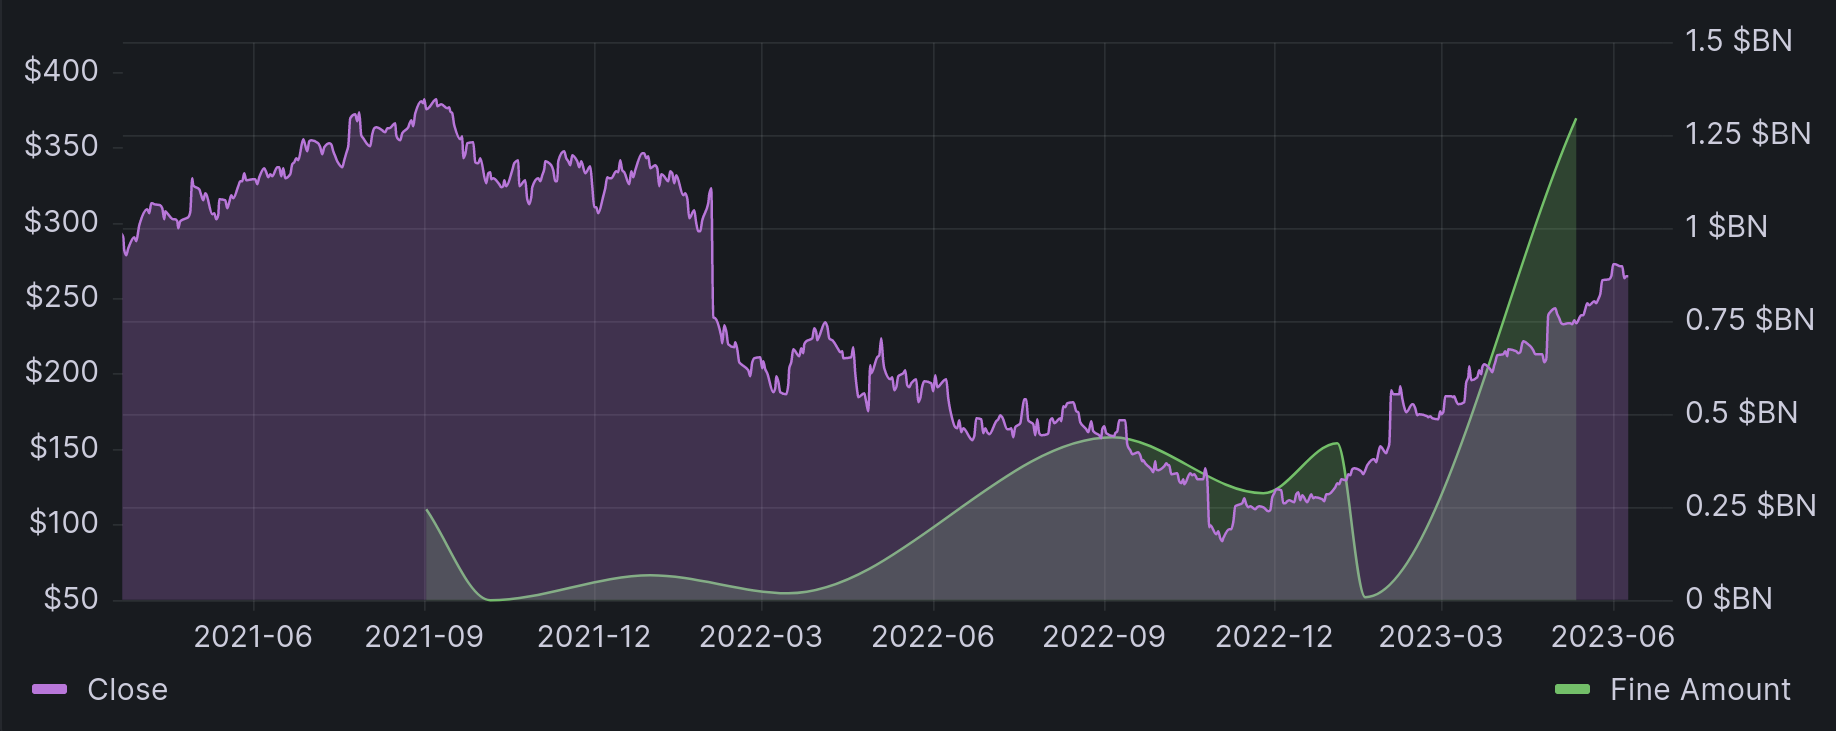
\includegraphics[width=1.00\textwidth]{rel-fines-stock-price}
    \caption{Comparison between Stock Price and Monetarial Amount of GDPR Fines}
    \label{fig:rel-stock-price}
\end{figure}

Likewise, the unchanged volume of shares traded signals no decrease in investor
confidence as displayed in Figure \ref{fig:volume}. Figure
\ref{fig:rel-fines-volume} below shows a comparison between the volume of shares
traded and the monetarial amount of GDPR fines.

\begin{figure}[H]
    \centering
    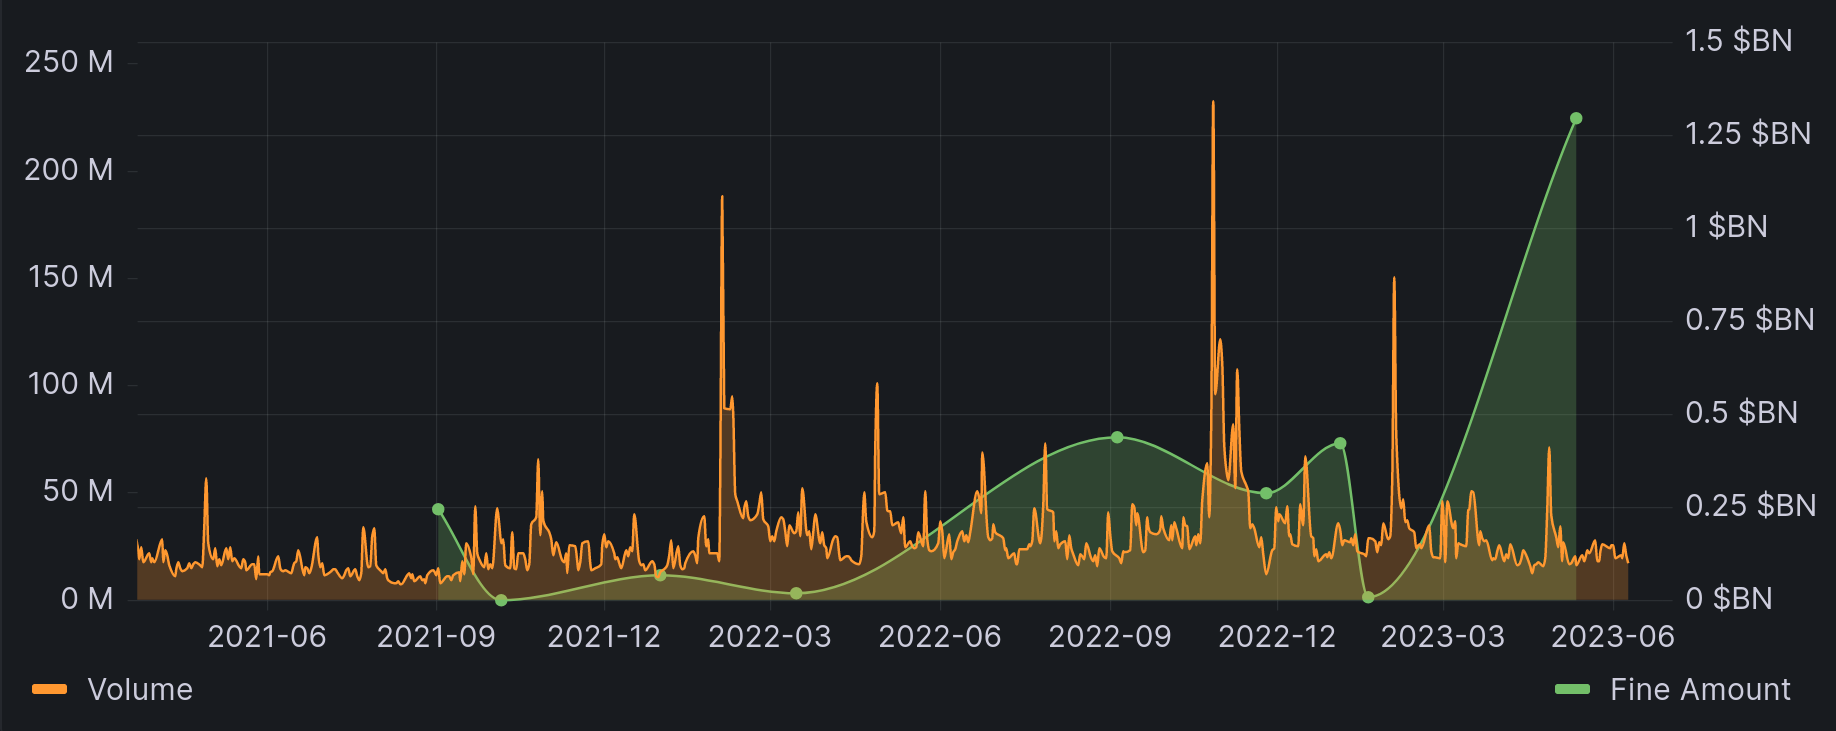
\includegraphics[width=1.00\textwidth]{rel-fines-volume}
    \caption{Comparison between Stock Volume and Monetarial Amount of GDPR Fines}
    \label{fig:rel-fines-volume}
\end{figure}

The average revenue per person shows no signs of correlation with the monetarial
amount of GDPR fines as shown in Figure \ref{fig:family-revenue-per-person}.

Dividing the average revenue per person by user geography region shows that
\textit{Meta's} revenue per person in Europe is less volatile than people in the
US despite Europe having nearly twice the users compared to the United
States\cite{2023q1}. The period from 31-Mar-2022 to 31-Dec-2022 is very
different from the rest of the timeline because a \%6.45 increase in revenue in
the US was met with a \%10.77 decline in revenue in Europe. Figure
\ref{fig:rel-fines-avg-revenue-per-person-region} below shows a comparison
between the average revenue per person by user geography region and the
monetarial amount of GDPR fines.

\begin{figure}[H]
    \centering
    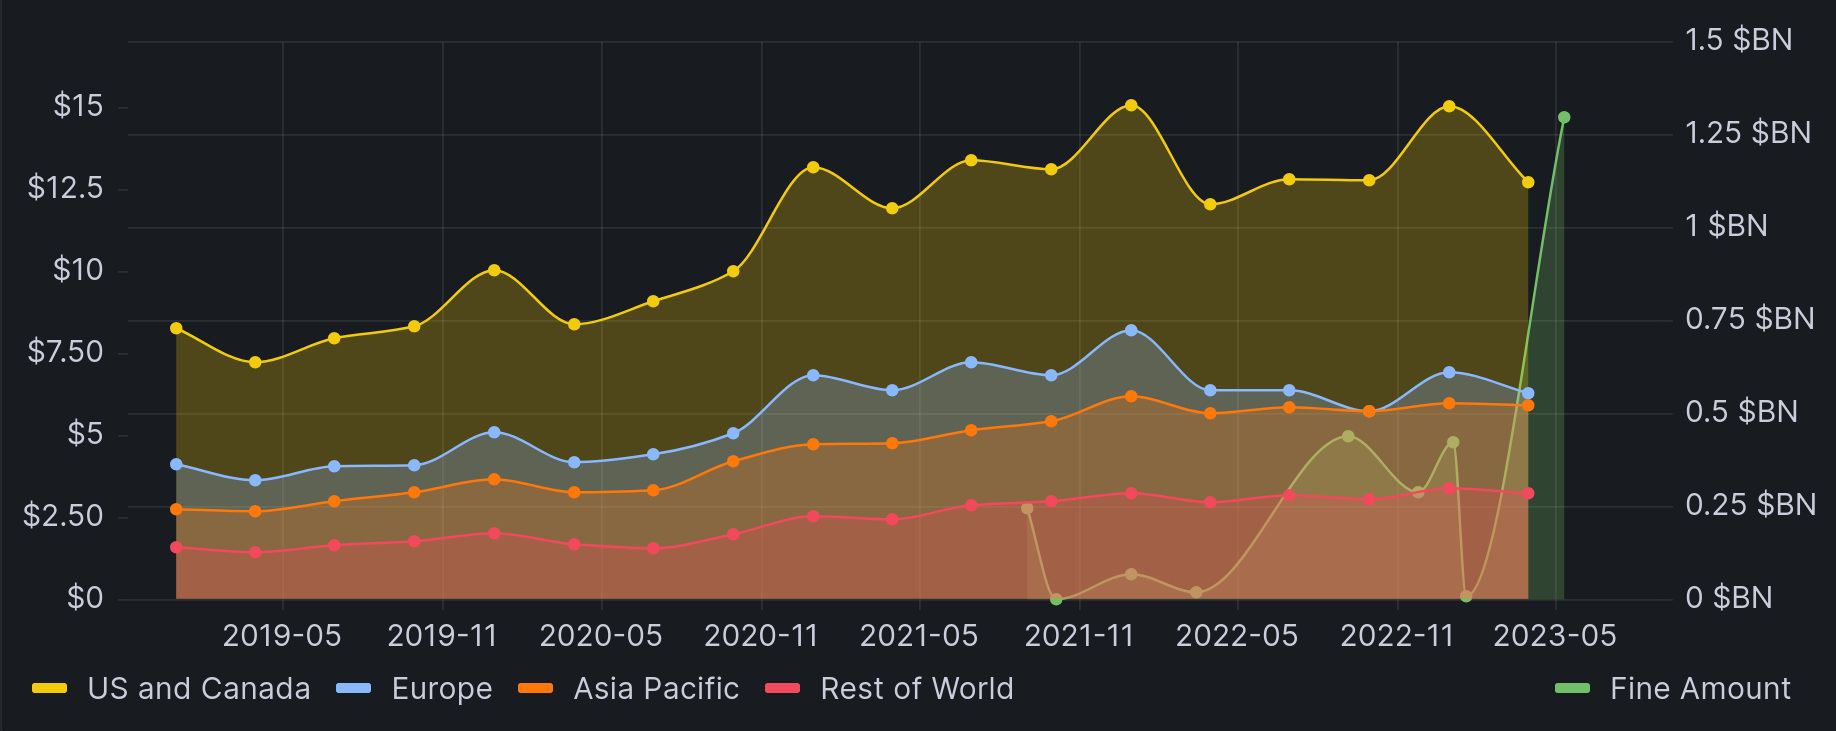
\includegraphics[width=1.00\textwidth]{rel-fines-avg-revenue-per-person-region}
    \caption{Comparison between Average Revenue per Person by User Geography Region and Monetarial Amount of GDPR Fines}
    \label{fig:rel-fines-avg-revenue-per-person-region}
\end{figure}

Figure \ref{fig:facebook-mau} and Figure \ref{fig:facebook-dau} show that the
number of daily and monthly active users in Europe has been steadily increasing
regardless of the fines imposed. It is worth noting that this increase seems to
be slowing down. Other regions show a similar trend with some showing a
shrinkage in the number of users.


The limitations of this study are that it does not consider the legal expenses
incurred by \textit{Meta Platforms, Inc.} in relation to GDPR non-compliance.
This includes expenses associated with hiring legal counsel, litigation,
settlement agreements, and any ongoing legal obligations. It also does not
consider the financial impact of reputational damage resulting from GDPR
non-compliance. Moreover, it does not investigate whether negative media
coverage, public backlash, or loss of user trust have affected \textit{Meta
Platforms'} brand value or customer perception. Further research could be done
into those areas.
\section*{Conclusion}

In conclusion, the fines imposed on \textit{Meta Platforms, Inc.} under the GDPR
have not had a substantial impact on the company's financial performance.
Investor confidence remains intact, as evidenced by the stability of the stock
price and trading volume around the time of the fines. Furthermore, the
company's revenue and net income have not been adversely affected by these
penalties. The only noticeable change is the less volatile average revenue per
person in Europe compared to the US. Especially in the period from 31-Mar-2022
to 31-Dec-2022 where a \%6.45 increase in revenue in the US was met with a
\%10.77 decline in revenue in Europe.

\bibliographystyle{vancouver}
\bibliography{refs}
\end{document}
